\documentclass{beamer}
\usetheme{CambridgeUS}

\usepackage{amsfonts}
\usepackage[utf8x]{inputenc}
\usepackage{listings}

\makeatletter
\def\BState{\State\hskip-\ALG@thistlm}
\makeatother

\lstdefinestyle{customc}{
  belowcaptionskip=1\baselineskip,
  breaklines=true,
  frame=L,
  xleftmargin=\parindent,
  language=Java,
  showstringspaces=false,
  basicstyle=\footnotesize\ttfamily,
  keywordstyle=\bfseries\color{red!40!black},
  commentstyle=\itshape\color{purple!40!black},
  identifierstyle=\color{black},
  stringstyle=\color{orange},
}
\lstset{escapechar=@,style=customc}

\setbeamertemplate{section page}
{
    \begin{centering}
    \begin{beamercolorbox}[sep=12pt,center]{part title}
    \usebeamerfont{section title}\insertsection\par
    \end{beamercolorbox}
    \end{centering}
}


\title{Java implemented Wiener attack simulation}
\subtitle{Cryptography Term Project}
\author{Gioacchino Castorio}
\institute{Università dell'Aquila}
\date{2017-06-20}
\begin{document}

\frame{\titlepage}

\begin{frame}{Table of contents}
\tableofcontents
\end{frame}

\section{RSA: an overview}

\frame{\sectionpage}


	\begin{frame}
    \frametitle{Story of RSA}
    \begin{itemize}
     	\item Invented in 1977 in MIT
     	\item Its name is made up from the initial letters the the surnames of the inventors (R. \textbf{R}ivest, A. \textbf{S}hamir and L. \textbf{A}dleman)
     	\item Its algorithm was under patent in US till 2000-09-06, altough it was publicly known
    \end{itemize}
  \end{frame}
  
  
  \begin{frame}
    \frametitle{Public-key (asymmetric) cryptography}
    % RSA è un metodo a chiave pubblica - chiave privata
    \begin{itemize}
    		\item The one who wants to receive encrypted messages \textbf{generates one pair of keys}: 
    		\begin{itemize}
    			\item a \textbf{public key} that is publicly retrievable
    			\item a \textbf{private key} that is kept secret by the owner
    		\end{itemize} 	 
    		\item This pair accomplish multiple function:
    		\begin{itemize}
    			\item \textbf{encryption}: a sender can use the public key to encrypt the message, while the owner can use the private key decrypt the incoming messages;
    			\item \textbf{authentication}: the public key could be used to verify that a holder of the corresponding private key sent the message (i.e. the owner ``signs" the message).
    		\end{itemize}
    \end{itemize}
  \end{frame}
  
  \begin{frame}
  \frametitle{RSA key generation algorithm}
    % descrizione generazione chiavi RSA
    
    \begin{enumerate}
    \item Choose \textbf{$p, q \in \mathbb{Z}$}, $p \neq q$ big primes;
    \item Compute $n = p \cdot q$ and $\phi(n) = (p-1) \cdot (q-1)$;
    \item Find $e \in \mathbb{Z}$, called ``\textbf{encryption exponent}", so that $1 \leq e < \phi(n)$ and $gcd(e, \phi(n)) = 1$;
    \item Find $d \in \mathbb{Z}$, called ``\textbf{decryption exponent}", so that $e \cdot d \equiv_{\phi(n)} 1$
    \item Now we can build the keys:
    \begin{itemize}
    	\item \textbf{Public key}: [\textbf{e}, n];
    	\item \textbf{Private key}: [\textbf{d}, q, p];
    \end{itemize}
    \end{enumerate}
    
  \end{frame}
  
  \begin{frame}
  \frametitle{RSA encrypt and decrypt method}
    % descrizione del metodo di crypt e decript
    Once the sender has retrieved the public key, he can easily encrypt a \textbf{plain message m}, such that $1 \leq m < n$:\\
    
    \begin{center}
    $c \equiv_n {m}^{e}$
    \end{center}
    
    Symmetrically, the owner of the private key that receives the \textbf{cipher text c} can obtain m:
    
    \begin{center}
    $ m \equiv_n {c}^{d} = {m}^{e \cdot d} \equiv {m}^{1}$
    \end{center}
    
  \end{frame}
	
	
\section{Attack RSA}

\frame{\sectionpage}


	\begin{frame}
 		 \frametitle{Why is RSA considered so secure?}
   		 % unica sicurezza del sistema: 
			% difficoltà di fattorizzazione dei numeri grandi
			% tutavia se si trova si riesce a trovare phi(n) si può fattorizzare facilmente
			
			\begin{itemize}
			\item Its security lies especially in the fact that it is very difficult (or roughly impossible) to \textbf{factorize very big integers} (represented as very long strings of bits);
			\item Big integer factorization is proved to be a \textbf{Not deterministic Polynomial} problem, although it might not be NP-complete
			\item It is fundamental to use p and q such that n would be made up of $\geq$ \textbf{1024 bits} (it takes years to be factorized)
			\end{itemize}
  		\end{frame}
  		
  \begin{frame}
  \frametitle{Wiener theorem}
    % teorema di Wiener (con dimostrazione?)
    \begin{itemize}
    	\item Given two primes p and q such that $q < p < 2q$;
    	\item Compute $n = p \cdot q$, $\phi(n) = (p-1) \cdot (q-1)$;
    	\item Given $1 < e,d < \phi(n)$ such that $e \cdot d \equiv_{\phi(n)} 1$;
    	\item If $d < \frac { 1 }{ 3 } { n }^{ \frac { 1 }{ 4 }  }$ then \textbf{d is simply computable}.
    \end{itemize}
    
  \end{frame}
  
  \begin{frame}
  \frametitle{Wiener attack algorithm}
  
  \begin{enumerate}
  
  \item Find the \textbf{$i^{th}$ convergent} (that we will call $\frac{A_i}{B_i}$) of $\frac { e }{ n }  \in  \mathbb{Q}$;
  \item If $C = \frac{e \cdot B_i - 1}{A_i} \in \mathbb{Z}$ then is C is a candidate for $\phi(n)$, otherwise return to \textit{step 1};
  \item If the equation ${x}^{2} - (n - C + 1)x + n = 0$ has integer solution $x_1, x_2$ then $x_1 = p$, $x_2 = q$, otherwise return to \textit{step 1}.
  
  \end{enumerate}
  
  \end{frame}
  		
\section{Java implementation of Wiener-vulnerable RSA}

  \frame{\sectionpage}
  
  \begin{frame}
  \frametitle{What is this project about?}
    % cosa insegna wiener? importanza di utilizzare una chiave di decrypt grande!
    It simulates a communication between a message sender and a receiver, using \textbf{1024 bit Wiener-vulnerable} $n = p \cdot q$ product on a single message block. After that, it simulates an attack against the public key with the Wiener algorithm (successful).
  \end{frame}
  
    \begin{frame}
    \frametitle{Project structure}
    
    The project consists essentially of a packaged RSA library built with:
    
    \begin{itemize}
    	\item Custom implemented classes:
    	\begin{itemize}
    		\item \textbf{IRSAChiper.java}: RSA Cipher interface and implementation;
    		\item \textbf{BigRational.java}: data structure for arbitrary dimension rational numbers representation (with operations);
    		\item \textbf{PublicKey.java} and \textbf{PrivateKey.java}: data structure that contains each part of the keys.
    	\end{itemize}
    	\item Default Java 8 SE classes:
    		\begin{itemize}
    			\item \textbf{BigInteger.java}: data structure for arbitrary dimension integer numbers representation (with operations like \textit{gcd}, \textit{power}, \textit{modulo}).
    		\end{itemize}
    	\end{itemize}
    
    
    
    
  
  \end{frame}
  
  
\begin{frame}
  \frametitle{IRSACipher.java interface [1/2]}
    % mostra l'interfaccia IRSAChiper e scrivi praticamente il javadoc
    
    \lstset{basicstyle=\tiny}
    \lstinputlisting[language=Java]{code/IRSACipher.java}
    
  \end{frame}
  
  \begin{frame}
  \frametitle{IRSACipher.java interface [2/2]}
  
  Essential method description:
    
    \begin{itemize}
    	\item \textbf{getWienerAttackableKeys}
    	\begin{itemize}
    		\item parameter \textit{factorlenght}: it is the bit length of the factors p and q, pseudo-randomly generated and tested by Rabin-Miller algorithm ($q < p < 2q$ checked);
    		\item it generates the decryption key d forcing it to be such that $bit(d) = bit[\frac{1}{3}{n}^{\frac{1}{4}}] - 1$ (Wiener is compulsorily respected);
    		\item it returns a \textit{KeyBundle} with the public and private keys of the owner.
    	\end{itemize}
    	
    	\item \textbf{attackWiener}
    	\begin{itemize}
    		\item parameter \textit{publicKey}: couple [e, n] to be attacked
    		\item it returns a \textit{KeyBundle} with the hacked public and private keys .
    	\end{itemize}
    \end{itemize}
    
  \end{frame}
  
  \begin{frame}
  \frametitle{BigRational.java [1/2]}
    % mostra l'interfaccia IRSAChiper e scrivi praticamente il javadoc
    
    \lstset{basicstyle=\tiny}
    \lstinputlisting[language=Java]{code/BigRational.java}
    
  \end{frame}
  
    \begin{frame}
  \frametitle{BigRational.java [2/2]}
    Essential method description:
   
   \begin{itemize}
   \item \textbf{getListIntegersContinuedFraction}
   \begin{itemize}
   		\item It decomposes the rational in $r = a_0 + r_1 = a_0 + \frac{1}{\frac{1}{r_1}}$;
   		\item It returns the list of ordered integers that make up the continued fraction expansion of the rational;
   \end{itemize}
   \item \textbf{recomposeConvergent} (\textit{static method})
   \begin{itemize}
   \item Retuns the ${n}^{th}$ convergent from  the passed integer list
   \end{itemize}
   \end{itemize}
    
  \end{frame}
  
  \begin{frame}
  
  \frametitle{Workflow [1/3]}
  
  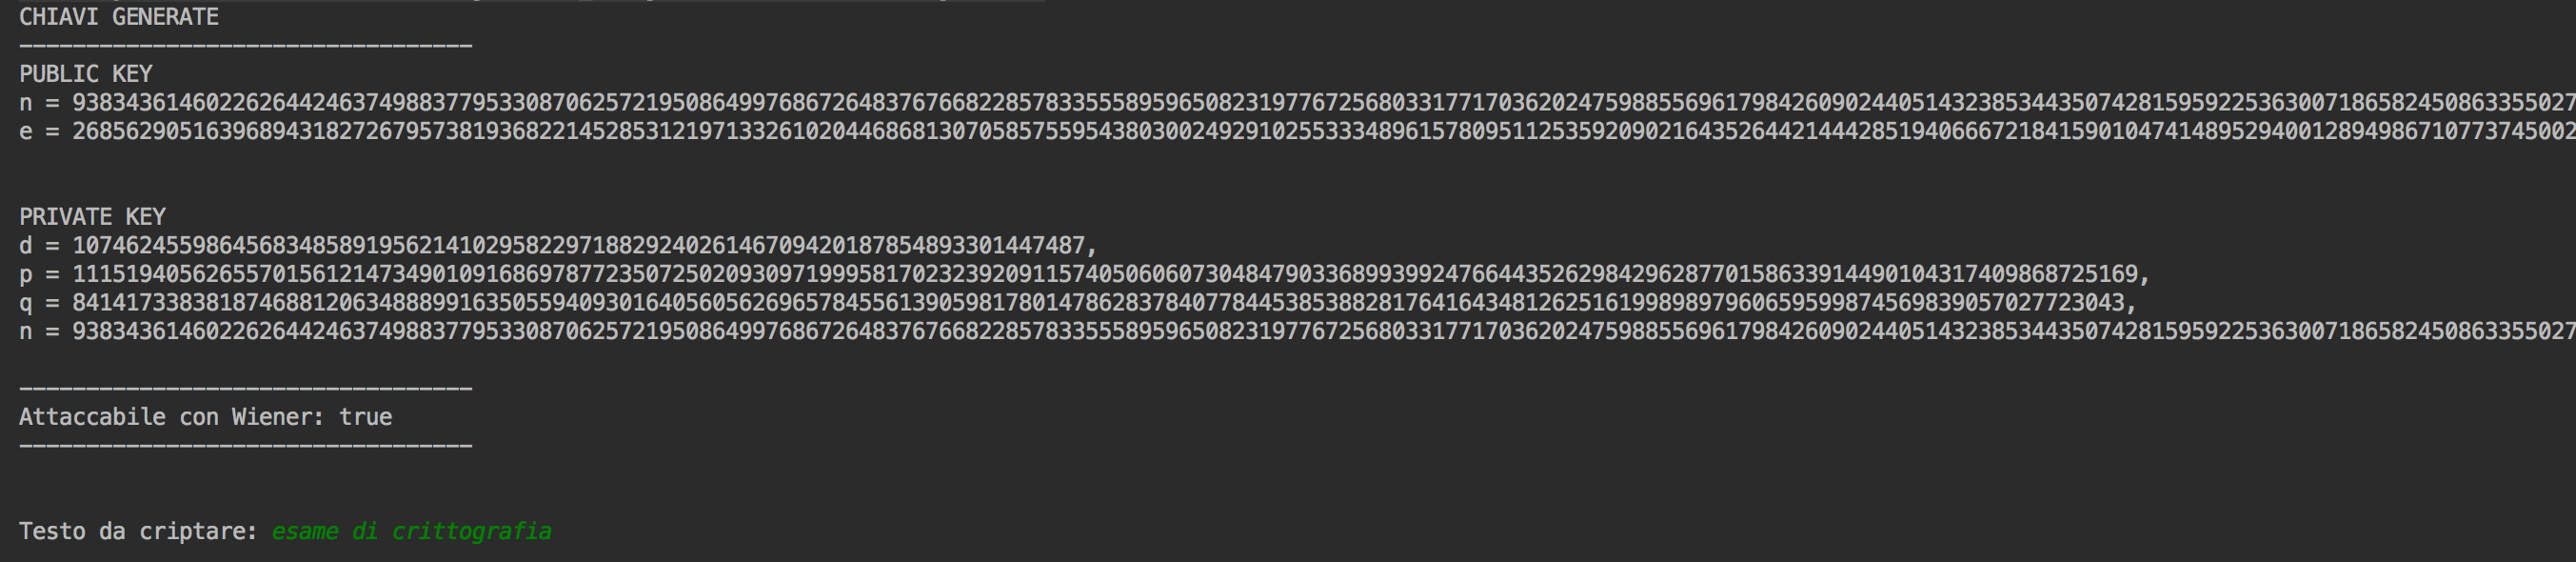
\includegraphics[height=3cm, width=12cm]{img/img_chiavi_generate}
  
  What does this image show:
 	\begin{enumerate}
 	\item The systems generates the key cuple and promts it;
 	\item It prompts the results of the Wiener vulnerability check;
 	\item The system requests the sender to write a message.
 	\end{enumerate}
 
  \end{frame}
  
    \begin{frame}
  
  \frametitle{Workflow [2/3]}
  
  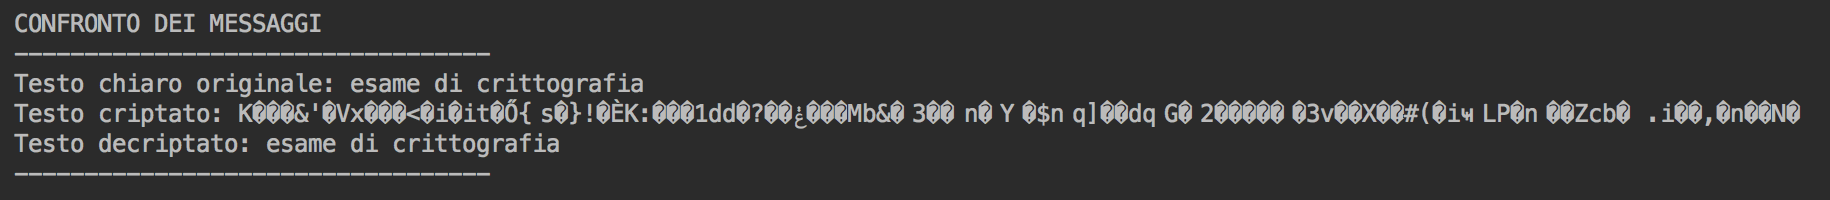
\includegraphics[height=2cm, width=12cm]{img/testo_criptato}
  
  Let's see these lines:
 	\begin{enumerate}
 	\item The plain message (not encrypted);
 	\item The chiper text (encrypted by the public key);
 	\item The result of the decryption (same as the plain message).
 	\end{enumerate}
 
  \end{frame}
  
    \begin{frame}
  
  \frametitle{Workflow [2/3]}
  
  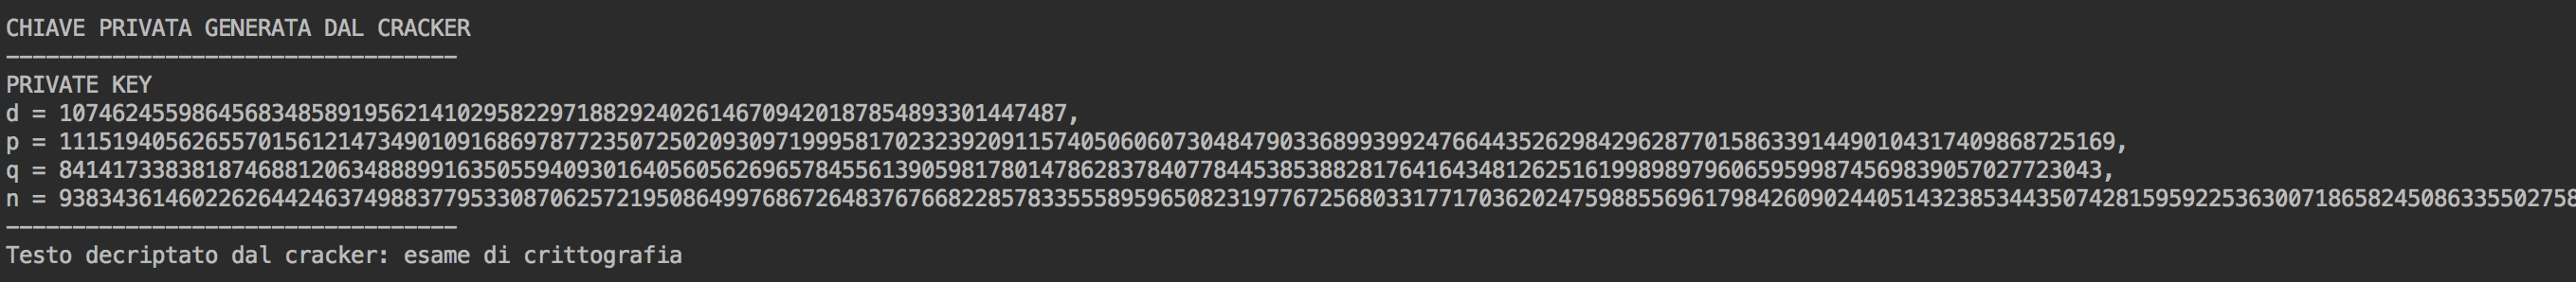
\includegraphics[height=2cm, width=12cm]{img/attacco}
  
  What has Eveline managed to do?
 	\begin{enumerate}
 	\item She has obtained the (p, q) cuple;
 	\item She has computed the \textbf{decription exponent} easely ($e \cdot d \equiv_{\phi(n)} 1$)!
 	\item She has decrypted the whole message!
 	\end{enumerate}
 
  \end{frame}
 
  
  \section*{}
  
    \begin{frame}
  % \frametitle{End}
    % cosa insegna wiener? importanza di utilizzare una chiave di decrypt grande!
    \begin{center}
           \textbf{Thank you for your attention}\\
           Let's try it!
    \end{center}
  \end{frame}


\end{document}